\documentclass[citation\_needed]{subfiles}
\begin{document}

L'outil d'annotation en EN de \Luxid\ s'appelle la TM360. Il fonctionne sur le principe de la cascade de transducteurs pour effectuer l'annotation, qui va enrichir le texte progressivement, via l'ajout de nouvelles informations (annotations) ou leur réécriture (désambiguisation). Les règles sont écrites via un format XML qui sera alors compilé, un exemple de règle est donné dans la figure\ \ref{fig:tm360-rule}. Elles manipulent en fait un graphe qui sera soit enrichi, dans le cas des annotations, ou simplifié, dans le cas des désambiguisations. La règle de la figure\ \ref{fig:tm360-rule} est illustrée sur la figure\ \ref{fig:tm360-application}.

\begin{figure}[ht!]
% \centering
% \lstset{language=XML}
% \begin{lstlisting}[basicstyle=\scriptsize]
% <annotation name="Entity" level="20">
  % <annotation name="Person">
     % <e priority="1">~~FirstName / ~~LastName</e>
     % <e priority="2">~~FirstName / \p:[A-Z][a-z]+</e>
  % </annotation>
% </annotation>
% \end{lstlisting}
\begin{xml}
\xmarker{annotation}{ \xfield{name}{Entity} \xfield{level}{20}}{\\
  \xmarker{annotation}{ \xfield{name}{Person}}{\\
     \xmarker{e}{ \xfield{priority}{1}}{\~{}\~{}FirstName / \~{}\~{}LastName}\\
     \xmarker{e}{ \xfield{priority}{2}}{\~{}\~{}FirstName / \textbackslash{}p:[A-Z][a-z]+}\\
  }\\
}
\end{xml}
\caption{un exemple de règle pour les outils Luxid. "\~{}\~{}" indique l'utilisation d'un dictionnaire. "/" est utilisé pour séparer les différents tokens. l'imbrication des balises annotation permet de créer des annotations hiérarchisées. "level" indique la n-ième passe de traitement. "priority" indique l'ordre de priorité de l'application des règles, si la priorité est fournie, une seule annotation sera produite par la règle.}
\label{fig:tm360-rule}
\end{figure}

La nature des informations ajoutées à un niveau donné peut se baser sur le contexte, la morphologie, ou provenir de dictionnaires. Chaque information ajoutée peut être utilisée dans les niveaux supérieurs afin de permettre l'annotation de concepts plus généraux ou la désambiguisation contextuelle de certains concepts ambigus. Par exemple, un nom de personne peut être ambigu avec une ville: \emph{Paris} qui est le nom de la capitale peut également être un prénom (féminin comme masculin) ou un nom de famille. Un lieu pouvant également être ambigu avec une organisation, dans le cas des pays notamment. La TM360 dispose également d'un processus appelé la propagation des annotations en entités nommées à l'échelle d'un document: si une entité à pu être identifiée de façon non ambigue à certains endroits du document mais pas à d'autres, la propagation va permettre d'annoter les entités manquées.

\begin{figure}[ht!]
\centering
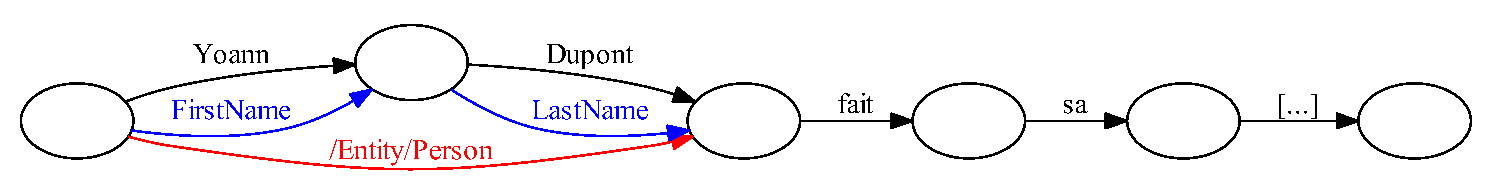
\includegraphics[scale=0.6]{images/Luxid/sentence1}
\caption{un exemple de réécriture de graphe selon la règle décrite dans la figure\ \ref{fig:tm360-rule}.}
\label{fig:tm360-application}
\end{figure}

\end{document}